\chapter{Arquitectura de Re-Volt America}
La arquitectura de Re-Volt America, a nivel de software y ambiente operacional, contempla diversas características que involucran tanto conocimientos técnicos como de Re-Volt y sus elementos propios.

A lo largo de las secciones de este capítulo, se detallará cómo Re-Volt America está construido desde el punto de vista de su arquitectura de software, y cómo todos sus componentes son orquestados para converger en el servicio que provee a sus usuarios.

Dentro de las diversas cosas que se detallarán están:
\begin{itemize}
  \item Paquete de Contenido de RVA.
  \item El repositorio de RVA-Data.
  \item Despliegue de servicios.
  \item Organización de GitHub.
  \item Servidor de distribución.
\end{itemize}

Al final de este capítulo, se concluirá sobre cómo el nuevo sistema desarrollado se integra a la arquitectura de RVA para poder funcionar de manera efectiva y ser lo menos  disruptiva posible.

\section{Organización de GitHub}
Como introducción general, las organizaciones de GitHub no son más que un conjunto de repositorios de Git. El dueño de la organización de GitHub puede definir ciertos roles y límites de acceso a determinados repositorios, así como también definir variables secretas para el despliegue de servicios, llaves criptográficas asociadas a la organización, dominios, entre otras características administrativas.

Re-Volt America cuenta con una organización de GitHub hace ya varios años. Haciendo uso de esta organización, ha conseguido mantener un control de los archivos y proyectos asociados a la comunidad.

Dentro de la organización, es posible encontrar los siguientes repositorios:

\begin{itemize}
  \item \textbf{Website}: Repositorio de la página web estática de RVA.
  \item \textbf{rva\_packs}: Repositorio para el paquete de contenido de RVA.
  \item \textbf{rva\_cars}: Sub-módulo de rva\_pack. Contiene todos los archivos de autos que se utilizan en RVA.
  \item \textbf{rva\_tracks}: Sub-módulo de rva\_pack. Contiene todos los archivos de pistas que se utilizan en RVA.
  \item \textbf{RVA-Data}: Repositorio de datos estáticos para el backend de RVA.
\end{itemize}

Todos estos repositorios funcionan de manera conjunta y son mantenidos por la administración de RVA.

A nivel organizacional, se cuenta con algunas variables secretas para el despliegue e integración continua que se deben tener en cuenta. Esta variables son definidas internamente en la organización de GitHub. Los flujos de trabajo de GitHub pueden hacer referencia a ellas agregando el prefijo ''\textit{secrets}''. Por ejemplo, \textit{secrets.FTP\_PASSWORD}.

\begin{center}
  \begin{tabular}{ | p{5cm} | p{10cm}| }
    \hline
    \multicolumn{2}{|c|}{\textbf{Variables Secretas RVA}} \\
    \hline
    \multicolumn{1}{|c|}{\textbf{Secreto}} & \multicolumn{1}{|c|}{\textbf{Detalle}} \\
    \hline
    {\textbf{FTP\_SERVER}} & URL del servidor de distribución. \\ \hline
    
    {\textbf{FTP\_PASSWORD}} & Contraseña del servidor FTP de distribución RVA. \\ \hline
    
    {\textbf{DEPLOY\_PASSWORD}} & Contraseña para descifrar la llave de despliegue de Capistrano. \\
    
    \hline
  \end{tabular}
\end{center}

\newpage

\section{Repositorios del Paquete de Contenido de RVA}
Como se explicó en la \autoref{problem:context:rva:pack}, RVA maneja un paquete de contenido de expansión para RVGL. Este paquete de contenido es versionado a través de Git en los repositorios de \textit{rva\_cars/} y \textit{rva\_tracks/}. Estos dos repositorios son sub-módulos del repositorio \textit{rva\_pack/}. Para integrar todos estos repositorios, se tiene un archivo \textbf{Rakefile}, el cual contiene las tareas necesarias para comprimir y desplegar el paquete de contenido de RVA.

El árbol de directorios del repositorio \textit{rva\_pack/} se puede ver en la \autoref{fig:rva_pack.png}.

\begin{figure}[H]
  \begin{center}
    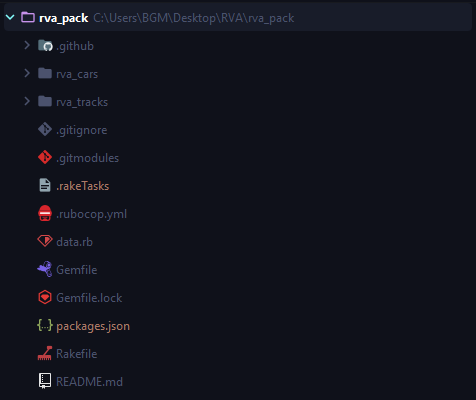
\includegraphics{rva_pack.png}
  \end{center}
  \caption[Árbol de directorios de rva\_pack]{Árbol de directorios de rva\_pack}
  \label{fig:rva_pack.png}
\end{figure}

Para versionar los paquetes, se utiliza un sistema basado en fechas. Por ejemplo, si la fecha es 30/10/2023, entonces ésta se traduce a la versión \textit{23.1030a-1}. El sufijo \textit{a-1} es simplemente una forma de diferenciar las versiones que fueron lanzadas en un mismo día.

\newpage

El versionado de todos los paquetes se encuentra en el archivo \textit{data.rb}, el cual se puede apreciar a continuación.

\begin{longlisting}
  \begin{minted}[mathescape,
    linenos,
    numbersep=5pt,
    breaklines,
    frame=single,
    framesep=2mm]{ruby}  
module RVA
  NAME = 'Re-Volt America'
  DESCRIPTION = "Re-Volt America's Official Content Pack"
  YEAR = 23
  MONTH = 10
  DAY = 30
  REVISION = 1
  SUFFIX = 'a'
  VERSION = "#{YEAR}.#{MONTH < 10 ? "0#{MONTH}" : MONTH}#{DAY < 10 ? "0#{DAY}" : DAY}#{SUFFIX}-#{REVISION}"
  
  module RVACars
    NAME = 'rva_cars'
    DESCRIPTION = "Re-Volt America's Cars Pack"
    YEAR = 23
    MONTH = 10
    DAY = 30
    REVISION = 1
    SUFFIX = 'a'
    VERSION = "#{YEAR}.#{MONTH < 10 ? "0#{MONTH}" : MONTH}#{DAY < 10 ? "0#{DAY}" : DAY}#{SUFFIX}-#{REVISION}"
    URL = 'https://distribute.rva.lat/rva/rva_cars.zip'
  end
  
  module RVATracks
    NAME = 'rva_tracks'
    DESCRIPTION = "Re-Volt America's Tracks Pack"
    YEAR = 23
    MONTH = 10
    DAY = 30
    REVISION = 1
    SUFFIX = 'a'
    VERSION = "#{YEAR}.#{MONTH < 10 ? "0#{MONTH}" : MONTH}#{DAY < 10 ? "0#{DAY}" : DAY}#{SUFFIX}-#{REVISION}"
    URL = 'https://distribute.rva.lat/rva/rva_tracks.zip'
  end
end
  \end{minted}
  \caption[Versionado de Paquetes de RVA]{Estructura de versiones de paquetes de RVA (\textit{data.rb})}
\end{longlisting}

\newpage

El procedimiento de compilación y despliegue de los paquetes es el siguiente:
\begin{enumerate}
  \item Se comprimen \textit{rva\_cars/} y \textit{rva\_tracks/} en \textit{rva\_cars.zip} y \textit{rva\_tracks.zip}, respectivamente.
  \item Se calcula un checksum para cada archivo comprimido.
  \item Se extraen las versiones de cada uno de los paquetes.
  \item Se genera una archivo JSON llamado \textit{packages.json}, el cual contiene toda la información del paquete de RVA en un formato interpretable por RVGL.
  \item El archivo \textit{package.json} es enviado, a través de FTP, al servidor de distribución de RVA (\textit{https://distribute.rva.lat}).
\end{enumerate}

Como ejemplo general, el archivo \textit{packages.json} contiene información como el nombre que engloba a los paquetes, ''Re-Volt America'' en este caso. También cuenta con una versión global (''23.1030a-1'') y versiones para cada uno de los paquetes. Todos los paquetes cuentan con una ''url'', la cual apunta a un archivo comprimido listo para ser descargado.

El archivo \textit{packages.json} compilado se ve de la siguiente manera:

\begin{longlisting}
  \begin{minted}[mathescape,
    linenos,
    numbersep=5pt,
    breaklines,
    frame=single,
    framesep=2mm]{json}  
{
  "name": "Re-Volt America",
  "version": "23.1030a-1",
  "packages": {
    "rva_cars": {
      "description": "Re-Volt America's Cars Pack",
      "version": "23.1030a-1",
      "checksum": "f8d552",
      "url": "https://distribute.rva.lat/rva/rva_cars.zip"
    },
    "rva_tracks": {
      "description": "Re-Volt America's Tracks Pack",
      "version": "23.1030a-1",
      "checksum": "8306f6",
      "url": "https://distribute.rva.lat/rva/rva_tracks.zip"
    }
  }
}
  \end{minted}
  \caption[Esquema de Paquetes RVGL]{Estructura JSON para la distribución de paquetes RVGL (package.json).}
\end{longlisting}

\newpage

\section{Repositorio de RVA-Data}
El repositorio de RVA-Data contiene toda la información estática de los modelos de autos y pistas del paquete de RVA en formato CSV. Estos son los archivos CSV que utilizará la plataforma desarrollada en este proyecto de título para realizar la importación de modelos a la base de datos. Este repositorio es mantenido manualmente por los administradores de la comunidad.

El sistema de versionado es exactamente el mismo que el que utiliza el paquete de contenido de RVA.

\begin{longlisting}
  \begin{minted}[mathescape,
    linenos,
    numbersep=5pt,
    breaklines,
    frame=single,
    framesep=2mm]{ruby}  
module RVAData
  YEAR = 23
  MONTH = 10
  DAY = 30
  REVISION = 2
  SUFFIX = 'a'
  VERSION = "#{YEAR}.#{MONTH < 10 ? "0#{MONTH}" : MONTH}#{DAY < 10 ? "0#{DAY}" : DAY}#{SUFFIX}-#{REVISION}"
end
  \end{minted}
  \caption[Esquema de versionado de RVA-Data]{Estructura de versionado de RVA-Data (\textit{data.rb})}
\end{longlisting}

\newpage

\section{Servidor de Distribución}
Re-Volt America cuenta con un servidor de distribución. En este servidor, se encuentra funcionando \textbf{vsftpd} (servidor FTP). Este servidor está configurado de tal manera que puede recibir conexiones ajenas y permite la descarga pública de archivos desde el mismo.

La URL en la que funciona este servidor es \textit{https://distribute.rva.lat/}. Todos los administradores cuentan con credenciales FTP para el servidor, con lo que pueden conectarse y realizar cambios manuales; sin embargo, para lo que respecta a la integración continua, existe el usuario \textbf{deploy} en la máquina. Este usuario cuenta también con su set de credenciales y puede subir archivos al servidor.

De esta forma, si se desea subir archivos al servidor mediante el protocolo FTP, basta con un usuario y contraseña.

\newpage

\section{Despliegue e Integración Continua}
El despliegue e integración continua funciona con GitHub Actions. En este contexto, GitHub utiliza un archivo YML para la configuración del despliegue.

\begin{longlisting}
  \begin{minted}[mathescape,
    linenos,
    numbersep=5pt,
    breaklines,
    frame=single,
    framesep=2mm]{yaml}  
name: deploy
on:
  push:
    branches:
      - production
jobs:
  deploy:
    runs-on: ubuntu-latest
      steps:
      - uses: actions/checkout@v1
      - name: Set up Ruby 2.7.3
        uses: ruby/setup-ruby@v1
        with:
          ruby-version: 2.7.3
      - name: Bundle gems
        run: |
          gem install bundler
          bundler install --jobs 4 --retry 3
      - name: Run Rake tasks
        run: |
          bundle exec rake
      - name: Prepare FTP directories
        run: |
          mkdir rva_data
          mv yml rva_data
          mv rva_data.json rva_data
      - name: Deploy via FTP
        uses: SamKirkland/FTP-Deploy-Action@4.3.0
        with:
          server: ${{ secrets.FTP_SERVER }}
          username: rva
          password: ${{ secrets.FTP_PASSWORD }}
          local-dir: "./rva_data/"
          server-dir: "rva_data/"
  \end{minted}
  \caption[Workflow de Despleigue]{Estructura de despliegue de RVA-Data (\textit{deploy.yml})}
\end{longlisting}

\newpage

Para el despliegue y la integración continua de todos los componentes de RVA, se cuenta con una rama llamada \textit{production} en los repositorios de rva\_pack y RVA-Data. Al enviarse cambios a esta rama, se gatilla el workflow listado anteriormente, haciendo llegar una nueva versión al servidor de distribución.